\documentclass{beamer}
\usepackage{graphicx}
\usepackage{color}
\usepackage{verbatim}
\usepackage{amsmath}
\usepackage{bm}
\usetheme{Frankfurt}
\usecolortheme{lily}

\newcommand{\xx}{\textbf{r}}

\title{A Classical Density-Functional Theory for Describing Water Interfaces}
\author{Jessica Hughes}
\date{October 11, 2011}

\setbeamertemplate{navigation symbols}{}

\begin{document}

\begin{frame}
  \titlepage
\end{frame}

\section{Introduction}
\subsection*{}

\begin{frame}{Why Water is Cool}
\framesubtitle{Some interesting and unusual properties}
\begin{itemize}
 \item <1-> Simple structure/geometry
 \vspace{0.2cm}
 \item <2-> Strong hydrogen bonds
 \vspace{0.2cm}
 \item <3-> High melting, boiling, and critical temperature 
 \vspace{0.2cm}
 \item <4-> Density maximum above the melting point
 \vspace{0.2cm}
 \item <5-> Large dielectric constant
 \vspace{0.2cm}
 \item <6-> Cheap, abundant, nontoxic
\end{itemize}
\end{frame}

\begin{frame}{Density Functional Theory}
The Hohenberg-Kohn
theorem allows us to write the ground state
energy in terms of a universal functional of the electron density and a separate
term including the external potential. \\
\vspace{0.5cm}
\pause
Mermin gives a
theorem extending that of Hohenberg and Kohn to nonzero temperatures:
\begin{equation}
  A(T) = \underset{n(\xx)}{min}\left\{ F[n(\xx),T] + \int V_{ext}(\xx) n(\xx)
d^3r\right\}
\end{equation}
This is the basis for classical DFT, where $n(\xx)$ is the density of molecules
instead of electrons.
\end{frame}

\begin{frame}{Statistical Associating Fluid Theory}
\framesubtitle{Why water needs special treatment}
 \begin{itemize}
  \item <1-> Simple fluids: characterized by van der Waals and weak electrostatic interations
  \item <2-> Water: strong hydrogen bonding and polar interactions
 \end{itemize}
\begin{columns}
 \column <3-> {.5\textwidth}
\begin{figure}
 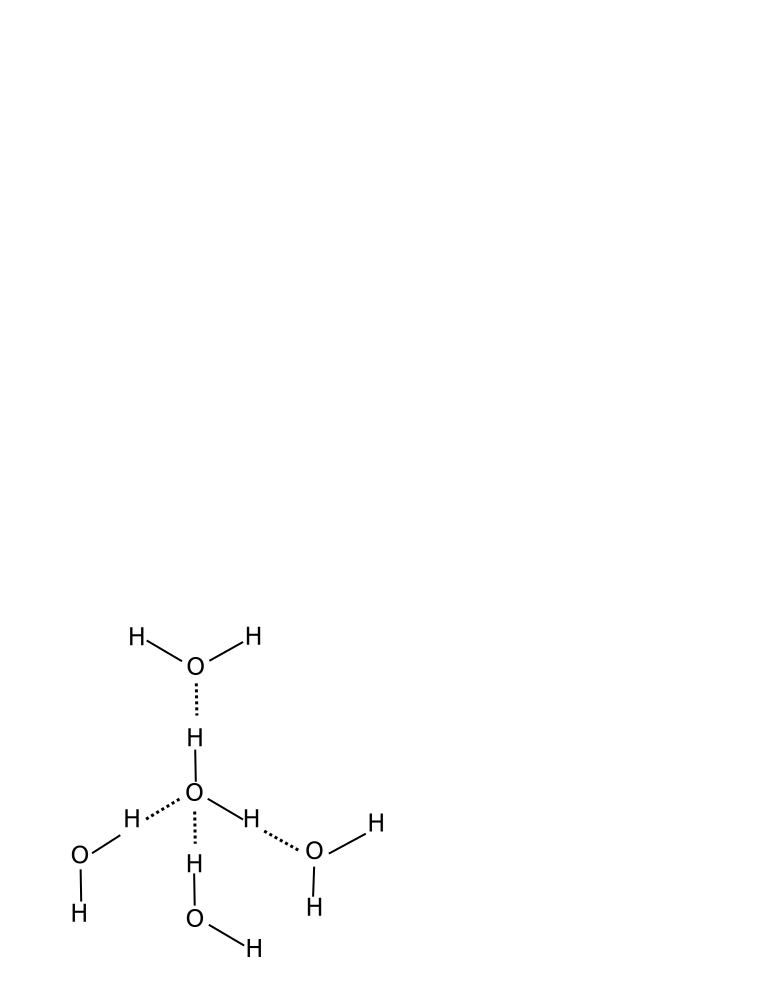
\includegraphics[width=4.2cm]{figs/hydrogen-bonding}
\end{figure}
\column <4-> {.5\textwidth}
Other examples of hydrogen-bonding fluids/molecules:\\
\begin{itemize}
 \item <4-> Alcohols
 \item <4-> Ammonia
 \item <4-> DNA
\end{itemize}
\end{columns}
\end{frame}

\begin{frame}{Statistical Associating Fluid Theory}
\vspace{0.7cm}
SAFT was designed for
use with fluids such as water, to account for the important association forces
as well as any effects due to clusters or chains forming
in the liquid.\\
\vspace{0.7cm}
\pause
Clark \emph{et al.}$^1$ have developed
a useful SAFT model for water that will be the basis for our functional in the
homogeneous limit.\\
\vspace{2cm}
\scriptsize{$^1$G.N.I. Clark, A.J. Haslam, A. Galindo, and 
G. Jackson.\\ \emph{Molecular Physics}, 104(22):3561-3581, 2006.}
\end{frame}

\section{The Functional}
\subsection*{}

\begin{frame}[fragile]{The Functional Terms}
The Helmholtz free energy functional is composed of:
\begin{equation}
  F[n] = F_\text{id}[n] + F_\text{hs}[n] + F_\text{disp}[n] + F_\text{assoc}[n] 
\end{equation}
where $F_\text{id}$ is the ideal gas free energy, $F_\text{hs}$ is
a hard-sphere free energy, $F_\text{disp}$ is the dispersion energy, and 
$F_\text{assoc}$ is the free energy of
association.
\end{frame}

\begin{frame}[fragile]{Ideal Gas Free Energy}
The ideal gas functional is given by
\begin{equation}
  F_{id}[n] = k_B T \int n(\xx)\left( \ln{\frac{n(\xx)}{n_Q}} - 1\right) d\xx
\end{equation}
where $n(\xx)$ is the density of water molecules and $n_Q$ is the
quantum concentration.
\begin{equation}
 n_Q =\left(\frac{mk_BT}{2\pi\hbar^2}\right)^{3/2}
\end{equation}
\end{frame}

\begin{frame}[fragile]{Hard-Sphere Free Energy}
\begin{itemize}
 \item <1-> For repulsive interactions, we use the White Bear version of
the Fundamental-Measure Theory~(FMT) functional.
 \vspace{0.5cm}
 \item <2-> This describes a hard-sphere fluid with a radius of $R=3.03420~\AA$
  (approximate size of a water molecule).
 \vspace{0.5cm}
 \item <3-> FMT functionals are expressed as the integral of
the \emph{fundamental measures} of a fluid.
  \begin{itemize}
    \item <4-> Filling fraction ($n_3$)
    \item <5-> Density of spheres touching a given point  ($n_2$)
  \end{itemize}
\end{itemize}
\end{frame}
 
\begin{frame}[fragile]{Dispersion Free Energy}
The dispersion free energy includes van der Waals attraction and 
any orientation-independent interactions. We use a
dispersion term based on the SAFT-VR approach, which has two free
parameters, an interaction energy $\epsilon_\text{d}$ and a 
length scale $\lambda_\text{d}$. It has the form
\begin{align}
  F_\text{disp}[n] &= \int (a_1(\xx) + \beta a_2(\xx))d\xx 
\end{align}
where $a_1$ and $a_2$ are the first two terms in a high-temperature
perturbation expansion.
\end{frame}

\begin{frame}[fragile]{Association Free Energy}
The association term models the hydrogen bonds as
four association sites on the surface of the
hard sphere. There is an attractive energy
$\epsilon_\text{assoc}$ when two molecules are arranged such that
the hydrogen of one interacts with the lone pair of the other.  The
volume of this interaction is $\kappa_\text{assoc}$ and the free 
energy is given by
\begin{align}  
  F_\text{assoc}[n] &= 4 k_BT \int n_0(\xx)\zeta(\xx)
  \left(\ln X(\xx) - \frac{X(\xx)}{2} + \frac12\right) d\xx
\end{align}
where the value of $4$ comes from the four association sites per
molecule, and the functional $X$ is the fraction of association sites
\emph{not} hydrogen-bonded. 
\end{frame}

\begin{frame}[fragile]{Empirical Parameters}
\framesubtitle{Fitting the functional to experiment}
There are five optimized parameters we take from Clark \emph{et al.}:
\begin{itemize}
 \item <2-> $R$ : hard sphere radius
 \item <3-> $\epsilon_\text{d}$ : dispersion interaction energy
 \item <4-> $\lambda_\text{d}$ : dispersion length scale
 \item <5-> $\epsilon_\text{assoc}$ : association attractive energy
 \item <6-> $\kappa_\text{assoc}$ : association interaction volume
\end{itemize}
\vspace{0.4cm}
\pause\pause\pause\pause\pause\pause
And one additional parameter we add:
\begin{itemize}
 \item <7-> $s_\text{d}$ : length scale for density averaging
\end{itemize}
\vspace{0.4cm}
\pause
These are optimized to fit experimental values such as vapor pressure, saturated 
liquid density, degree of association, and surface tension.
\end{frame}

\section{Thermodynamic Calculations}
\subsection*{}

% \begin{frame}[fragile]{Pressure Calculation}
% The pressure is obtained by taking a partial
% derivative with respect to volume at fixed temperature.  Since
% \emph{volume} isn't a parameter in density-functional theory, we
% consider the \emph{free energy per unit volume}.
% \begin{align}
%   F[n] &= f[n]V \\
%   p[n] &= -\left(\frac{\partial F[n]}{\partial V}\right)_{T} \\
%   &= -\left(\frac{\partial f[n]V}{\partial V}\right)_{T} \\
%   &= -V\left(\frac{\partial f[n]}{\partial V}\right)_{T}
%    - f[n]\left(\frac{\partial V}{\partial V}\right)_{T} \\
%   &= n \left(\frac{\partial f[n]}{\partial n}\right)_{T} - f[n]
% \end{align}
% \end{frame}

\begin{frame}[fragile]{Additional Thermodynamic Quantities}
In addition to Helmholtz free energy, we can easily calculate
\begin{align}
  p[n] &= -\left(\frac{\partial F[n]}{\partial V}\right)_{T} 
    = -\left(\frac{\partial f[n]V}{\partial V}\right)_{T} \nonumber \\
  &= n \left(\frac{\partial f[n]}{\partial n}\right)_{T} - f[n] \\
  S[n] &= \left(\frac{\partial F[n]}{\partial T}\right)_{V} \\
  U[n] &= F[n] + TS[n] \\
  H[n] &= F[n] + TS[n] + pV
\end{align}
\pause
One simple calculation: 
\begin{itemize}
 \item Heat of vaporization at atmospheric pressure is
$\Delta H_{vap}$=~39.41~kJ/mol (NIST: 40.65~kJ/mol).
\end{itemize}
\end{frame} 

\begin{frame}[fragile]{Temperature Coexistence Curve}
\begin{figure}
\begin{center}
\includegraphics[width=\columnwidth]{figs/temperature-versus-density}
\end{center}
\end{figure}
\end{frame}

\begin{frame}[fragile]{Determining Densities with the Common Tangent Rule}
\framesubtitle{At room temperature (298 K)}
\begin{figure}
\begin{center}
\includegraphics[width=\columnwidth]{figs/finding-vapor-pressure}
\end{center}
\end{figure}
\end{frame}

\begin{frame}[fragile]{Determining Densities with the Common Tangent Rule}
\framesubtitle{Close to the critical temperature}
\begin{figure}
\begin{center}
\includegraphics[width=\columnwidth]{figs/near-critical-point}
\end{center}
\end{figure}
\end{frame}

\begin{frame}[fragile]{Pressure Isotherms and Coexistence Curve}
\begin{figure}
\begin{center}
\includegraphics[width=\columnwidth]{figs/pressure-with-isotherms}
\end{center}
\end{figure} 
\end{frame}

% \begin{frame}[fragile]{Vapor Pressure - Cut this slide?}
% \begin{figure}
% \begin{center}
% \includegraphics[width=\columnwidth]{figs/equation-of-state}
% \end{center}
% \end{figure}
% \end{frame}

\begin{frame}[fragile]{Surface Tension}
\framesubtitle{Fit for liquid water near room temperature and 
atmospheric pressure using $s_\text{d}$}
\begin{figure}
\begin{center}
\includegraphics[width=\columnwidth]{figs/surface-tension}
\end{center}
\end{figure} 
\end{frame}

\section{Results: Slit}
\subsection*{}

% \begin{frame}[fragile]{Liquid-Vapor Interface}
% \begin{figure}
% \begin{center}
% \includegraphics[width=\columnwidth]{figs/surface-298}
% \end{center}
% \end{figure} 
% \end{frame}

\begin{frame}[fragile]{Water Constrained to a Slit}
\framesubtitle{One dimensional problem}
\begin{columns}
 \column {0.5\textwidth}
  \begin{figure}
  \begin{center}
  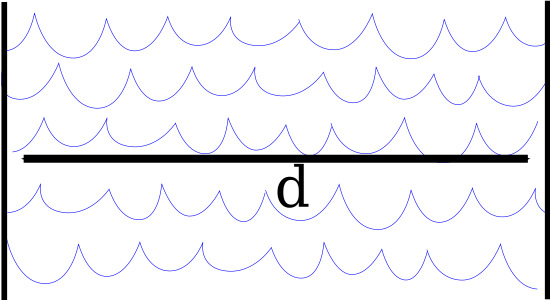
\includegraphics[width=4.5cm]{figs/slit-diagram}
  \end{center}
  \end{figure}
  Diagram of the water-filled slit.
 \column {0.5\textwidth}
  Setting up calculations for the slit:
  \begin{itemize}
  \item Pressure = 1~atm
  \item Temperature = 298~K
  \item Lattice spacing $\approx$~0.01~nm 
  \item Small non-zero density constraint outside the slit
  \item Slit size = 0.1~nm to 8~nm
  \end{itemize}
\end{columns}
\vspace{0.8cm}
We minimize the energy and calculate density, free energy, entropy, 
internal energy, and $X$.
\end{frame}

\begin{frame}[fragile]{Water Constrained to a Slit}
\framesubtitle{Density profile for 4~nm slit}
\begin{figure}
\begin{center}
\includegraphics[width=\columnwidth]{figs/density-1D}
\end{center}
\end{figure} 
\end{frame}

\begin{frame}[fragile]{Water Constrained to a Slit}
\framesubtitle{Hydrogen bonding in a 4~nm slit}
\begin{figure}
\begin{center}
\includegraphics[width=\columnwidth]{figs/xassoc-1D}
\end{center}
\end{figure} 
\end{frame}

\begin{frame}[fragile]{Water Constrained to a Slit}
\framesubtitle{Metastability}
Is it really possible to have liquid water in these nanoscale slits?
\vspace{0.5cm}
\begin{itemize}
 \item <2-> For slits smaller than 0.6~nm, the initial liquid water inside will
vaporize.
 \vspace{0.5cm}
 \item <3-> Will the larger slits containing liquid water be stable?
  \begin{itemize}
    \item <4-> Work to pull apart two hard walls = $10^{-7} - 10^{-8}$ Htr
    \item <4-> Free energy of liquid-filled slit = $10^{-5} - 10^{-6}$ Htr
  \end{itemize}
 \vspace{0.5cm}
 \item <5-> For the range of slit sizes we
studied, all the computational results of liquid-filled slits are
metastable.  
\end{itemize}
\end{frame}

\section{Results: Rods}
\subsection*{}

\begin{frame}{Hydrophobic Rods in Water}
\framesubtitle{Single rod diagram}
\begin{columns}
 \column {0.5\textwidth}
  \begin{figure}
  \begin{center}
  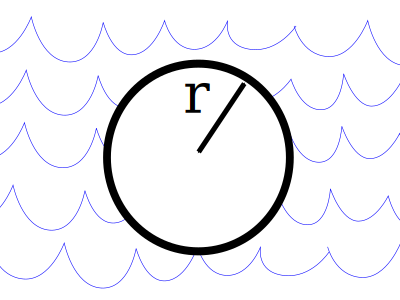
\includegraphics[width=4.5cm]{figs/single-rod-diagram}
  \end{center}
  \end{figure}
  Cross section diagram of a single hydrophobic rod in water.
 \column {0.5\textwidth}
  Setting up calculations for the rod:
  \begin{itemize}
  \item Pressure = 1~atm
  \item Temperature = 298~K
  \item Lattice spacing $\approx$~0.01~nm 
  \item Small non-zero density constraint outside the rod
  \item Radius = 0~nm to 1.5~nm
  \end{itemize}
\end{columns}
\vspace{0.5cm}
We minimize the energy and calculate density, free energy, entropy, 
internal energy, and $X$.
\end{frame}

\begin{frame}[fragile]{Hydrophobic Rods in Water}
\framesubtitle{Density profiles for single rods of various radius}
\begin{figure}
\begin{center}
\includegraphics[width=\columnwidth]{figs/density-single-rod}
\end{center}
\end{figure}
\end{frame}

\begin{frame}[fragile]{Hydrophobic Rods in Water}
\framesubtitle{Hydrogen bonding outside a slit of radius 0.2~nm}
\begin{figure}
\begin{center}
\includegraphics[width=\columnwidth]{figs/xassoc-single-rod}
\end{center}
\end{figure} 
\end{frame}

\begin{frame}[fragile]{Hydrophobic Rods in Water}
\framesubtitle{Total free energy per area for all radii}
\begin{figure}
\begin{center}
\includegraphics[width=\columnwidth]{figs/energy-vs-diameter}
\end{center}
\end{figure} 
\end{frame}

\begin{frame}[fragile]{Hydrophobic Rods in Water}
\framesubtitle{Resolution and convergence testing for a rod with radius 0.5~nm}
\begin{figure}
\begin{center}
\includegraphics[width=7.7cm]{figs/density-vs-radius}
\end{center}
\end{figure} 
\footnotesize{Resolutions:}
\begin{itemize}
 \item \footnotesize{High $\approx$ 0.003~nm (0.05 bohrs)}
 \item \footnotesize{Medium $\approx$ 0.01~nm (0.2 bohrs)}
 \item \footnotesize{Low $\approx$ 0.03~nm (0.5 bohrs)}
\end{itemize}
\end{frame}

\begin{frame}[fragile]{Hydrophobic Rods in Water}
\framesubtitle{Two rods diagram}
Cross section diagram of two rods in water.
\begin{figure}
\begin{center}
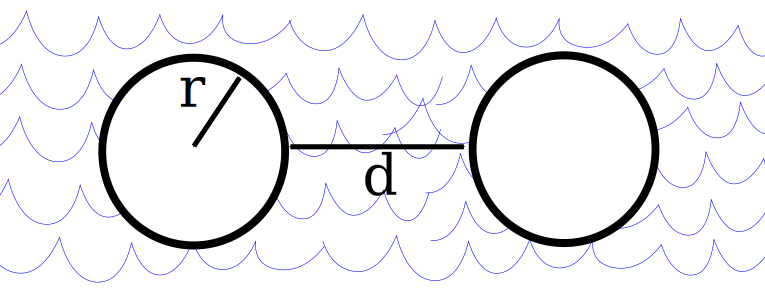
\includegraphics[width=\columnwidth]{figs/rods-diagram}
\end{center}
\end{figure}
The radius $r$ ranges from 0.1~nm to 1.0~nm and the separation
$d$ ranges from 0~nm to about 1.2~nm.
\end{frame}

\begin{frame}[fragile]{Hydrophobic Rods in Water}
\framesubtitle{Density profiles for two rods of radius 0.5~nm}
\begin{columns}
 \column{0.7\textwidth}
  \begin{figure}
  \includegraphics[width=7.3cm]{figs/density-rods-in-water}
  \end{figure} 
 \column{0.3\textwidth}
 \small{``Stadium''-shaped vapor-filled area between rods}\\
 \vspace{0.3cm}
 \small{$d=$~0.2~nm}\\
 \vspace{1.4cm}
 \small{Liquid-filled area between two rods}\\
 \vspace{0.3cm}
 \small{$d=$~0.6~nm}
\end{columns}
\end{frame}

\begin{frame}[fragile]{Hydrophobic Rods in Water}
\framesubtitle{Energies for rods of radius 0.5~nm}
\begin{figure}
\begin{center}
\includegraphics[width=\columnwidth]{figs/energy-rods}
\end{center}
\end{figure} 
\end{frame}

\begin{frame}[fragile]{Hydrophobic Rods in Water}
\framesubtitle{Free energy per length for all radii}
\begin{figure}
\begin{center}
\includegraphics[width=\columnwidth]{figs/rods-energy-vs-distance}
\end{center}
\end{figure} 
\end{frame}

\begin{frame}[fragile]{Hydrophobic Rods in Water}
\framesubtitle{The force per length}
  \begin{figure}
  \includegraphics[width=6.7cm]{figs/rods-energy-vs-distance}
  \end{figure}  
The force per length is constant, and surprisingly 
independent of separation. By finding the slope of this curve, we 
calculate this force per length to be 144~mN/m.
\end{frame}

\begin{frame}[fragile]{A Macroscopic Surface Tension Model}
\framesubtitle{Explaining the constant force per length for small separation}
\begin{itemize}
 \item <1-> Free energy of the rods = surface area times surface tension
 \item <2-> Free energy per length = circumference times surface tension
 \item <3-> Force per length = derivative of free energy per length with respect to the separation 
 \item <4-> We approximate the circumference of the stadium-shape by
  \begin{equation}
  C_{s} = 2\pi r +4r+2d
  \end{equation}
 \item <5-> Force per length = 2 times the surface tension
 \begin{itemize}
  \item <6-> Fitted surface tension for bulk water = 72 mN/m
  \item <6-> Free energy per area asymptote for single rods = 75 mN/m
  \item <6-> Force per length from slope = 144~mN/m
 \end{itemize}
\end{itemize}
\end{frame}

\begin{frame}[fragile]{Vapor-Liquid Transition}
\framesubtitle{Estimating the critical separation} 
Using the same macroscopic surface tension model, we propose that 
the critical separation, $d_c$, will occur when the free energies are equal. This 
corresponds to equating the circumference of the stadium-shape and the circumference of the two rods, which results in
\pause
\begin{align}
C_\text{stadium} &= C_\text{rods} \\
2\pi r +4r+2d_c &= 4\pi r \\
d_c &= (\pi-2)r
\end{align}
\end{frame}

\begin{frame}[fragile]{Vapor-Liquid Transition}
\framesubtitle{The critical separation results}
The results for estimating the critical separation for the vapor-liquid 
transition.
\begin{table}
\begin{tabular} {|c|c|c|c|}
\hline
$r$ (nm) & $d_c$ prediction (nm) & $d_c$ result (nm) & \% error \\
\hline
0.3 & 0.34 & 0.23 & 32\% \\
\hline
0.5 & 0.57 & 0.54 & 5.3\% \\
\hline
0.7 & 0.80 & 0.81 & 1.3\% \\
\hline
0.9 & 1.03 & 1.06 & 2.9\% \\
\hline
1.0 & 1.14 & 1.19 & 4.4\% \\
\hline
\end{tabular}
\end{table}
\pause 
The diameter of a water molecule is approximately 0.6~nm.\\
\vspace{0.5cm}
\pause
This relation will not hold for all radii rods, it will 
likely become a gradual transition for very large rods.
\end{frame}

\section{Conclusions}
\subsection*{}

\begin{frame}[fragile]{Hydrophobic Interactions}
\begin{itemize}
 \item <1-> Two hydrophobic rods in water will transition from vapor to liquid between the rods.
 \vspace{0.5cm}
 \item <2-> This transition can be approximated with a macroscopic surface tension model
  for rods larger than 0.5~nm.
 \vspace{0.5cm}
 \item <3-> The separation necessary for the transition is $d_c = (\pi-2)r$.
 \vspace{0.5cm}
 \item <4-> The computationally efficient functional produces reasonable results for
hydrophobic interations.
\end{itemize}
\end{frame}

\begin{frame}[fragile]{Future Work}
\framesubtitle{Using the functional for more complex interactions}
\begin{itemize}
 \item <1-> More configurations of hydrophobic rods
 \vspace{0.5cm}
 \item <2-> Hydrophobic spheres
 \vspace{0.5cm}
 \item <3-> Hydrophilic solutes
\end{itemize}
\end{frame}

\begin{frame}{Thanks for Listening...}
\begin{center} 
\huge{Questions?}
\end{center}
\end{frame}

\end{document}
